\documentclass{letter}
\usepackage{geometry}
\usepackage{graphicx}

\begin{document}
\begin{letter}{}
  \opening{Dear Editor:}

  We are submitting a manuscript, ``The Magnetorotational Instability Prefers Three Dimensions,'' for consideration in \emph{Nature Physics}.
The magnetorotational instability (MRI) is an extremely important part of astrophysical fluid dynamics, as it is believed to play a key role in accretion disks around compact objects and may also play an important role in stellar interiors.
There are several active laboratory campaigns to make an experimental confirmation of the instability.
Our work demonstrates for the first time that the MRI is three-dimensional at onset when the shear that drives it is close to its critical value.
Far from being an unusual part of parameter space, driving the flow to near-critical shear is how the instability saturates in systems like stars and laboratory experiments, similar to convection driving the background entropy gradient to zero or Taylor-Couette instability forcing the angular momentum gradient toward a stable profile.
This means that in the context of stellar interiors and the laboratory experiments seeking to confirm the existence of the MRI, near-critical shear is in fact a very important regime.
The implication of a three-dimensional MRI are twofold: the non-normal nature of the linear operator driving the instability implies that transient growth is always important in the linear phase.
More importantly, the existance of a three-dimensional unstable mode implies that the MRI may drive dynamo action, amplifying magnetic fields even in the absence of turbulence driven by secondary instabilities.

Our results have important implications for both laboratory studies of the MRI as well as its effects in stellar interiors. 
The MRI is also an important magnetohydrodynamic process in its own right: it is of interest to plasma physicists and it bears deep connections to viscoelastic Taylor-Couette flow that have been studied in the fluid dynamics community. 
Thus, because our work constitutes an important new direction in MRI research, we believe it is well suited for the diverse readership of \emph{Nature Physics}. We look forward to corresponding further with you about our work.

\closing{Sincerely, \\
\fromsig{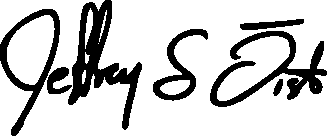
\includegraphics[scale=0.5]{jso_sig.pdf}}\\
\fromname{Jeffrey S. Oishi,\\on behalf of the authors:\\
Geoffrey M.\ Vasil\\
Morgan Baxter\\
Andrew Swan\\
Keaton J. Burns\\
Daniel Lecoanet\\
Benjamin P. Brown}}

\end{letter}
\end{document}

